\documentclass{article}
\usepackage[utf8]{inputenc}

\title{CS246 Homework 3 Answers}
\author{Charlie Zhang}
\date{Feb 2013}

\usepackage{natbib}
\usepackage{float}
\usepackage{graphicx}
 \usepackage{indentfirst}
\usepackage{mathtools}
\usepackage{setspace}
\linespread{1.8}
\newenvironment{myenv}[1]
  {\begin{spacing}{#1}}
  {\end{spacing}}
  
\begin{document}

\maketitle
\section{Question 1 -- Latent Features for Recommendations}


\subsection{(a)}
$\epsilon_{iu} = r_{iu} - q_i * p_u^T$

$q_i \leftarrow q_i + \eta(\epsilon_{iu}p_u - \lambda q_i)$

$p_u \leftarrow p_u + \eta(\epsilon_{iu}q_i - \lambda p_u)$

Where $\eta$ is the learning rate.

\subsection{(b)}
\begin{figure}[H]
\centering
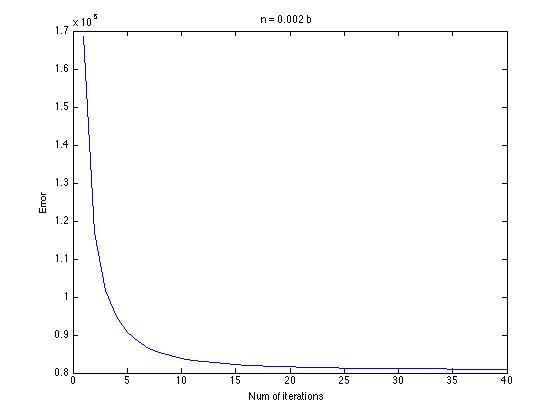
\includegraphics[scale=0.5]{EAsOfIterationEta0002.jpg}
\caption{ Error in first 40 iterations with $\eta=0.002$: }
\label{}
\end{figure}


\subsection{(c)}
\begin{figure}[H]
\centering
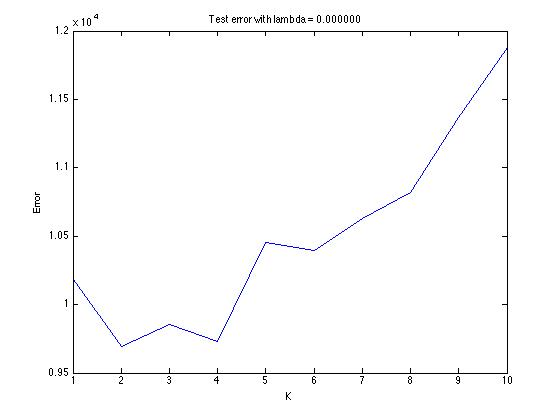
\includegraphics[scale=0.5]{TestErrorLambda0.jpg}
\caption{ $E_{te}$ as of K with $\lambda=0.0$:}
\label{}
\end{figure}

\begin{figure}[H]
\centering
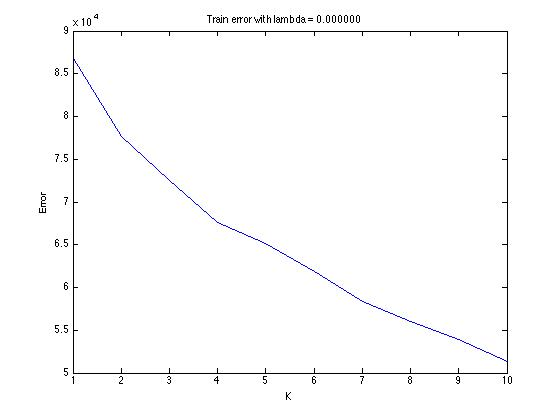
\includegraphics[scale=0.5]{TrainErrorLambda0.jpg}
\caption{ $E_{tr}$ as of K with $\lambda=0.0$:}
\label{}
\end{figure}

\begin{figure}[H]
\centering
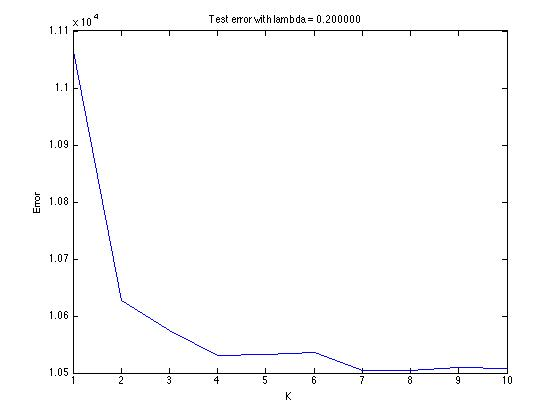
\includegraphics[scale=0.5]{TestErrorLambda02.jpg}
\caption{ $E_{te}$ as of K with $\lambda=0.2$:}
\label{}
\end{figure}

\begin{figure}[H]
\centering
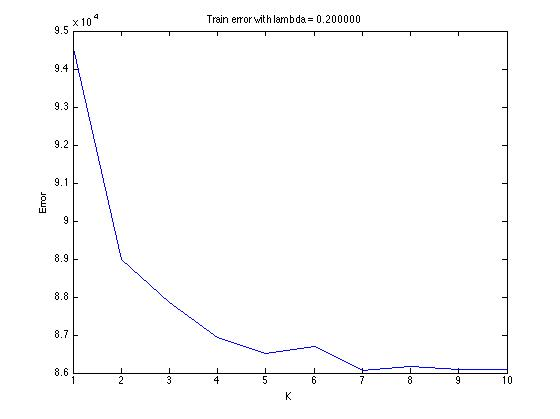
\includegraphics[scale=0.5]{TrainErrorLambda02.jpg}
\caption{ $E_{tr}$ as of K with $\lambda=0.2$:}
\label{}
\end{figure}

True statements are: \textbf{B, D, H}


\subsection{(d)}
Update model as:\\
$R_{iu} = \mu + b_u + b_i + q_i\cdot p_u^T$ \\

The update equations are:\\
$\epsilon_{iu} = r_{iu} - \mu - b_u - b_i - q_i * p_u^T$

$q_i \leftarrow q_i + \eta(\epsilon_{iu}p_u - \lambda q_i)$

$p_u \leftarrow p_u + \eta(\epsilon_{iu}q_i - \lambda p_u)$

$b_i \leftarrow b_i + \eta(\epsilon_{iu} - \lambda b_i)$

$b_u \leftarrow b_u + \eta(\epsilon_{iu} - \lambda b_u)$

Where $\eta$ is the learning rate.

And plot the following:\\

\begin{figure}[H]
\centering
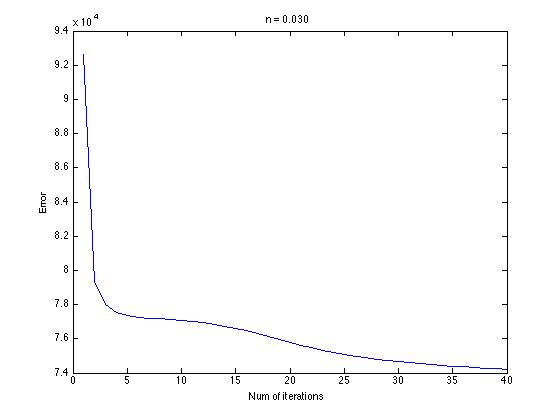
\includegraphics[scale=0.5]{EAsOfK-V2.jpg}
\caption{ Error in first 40 iterations with $\eta=0.03$: }
\label{}
\end{figure}

\begin{figure}[H]
\centering
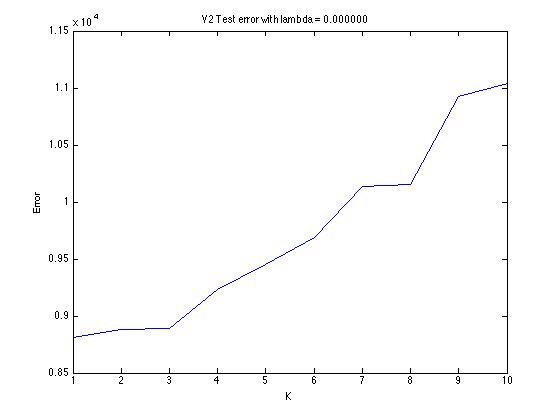
\includegraphics[scale=0.5]{TestErrorLambda0-V2.jpg}
\caption{ $E_{te}$ as of K with $\lambda=0.0$:}
\label{}
\end{figure}

\begin{figure}[H]
\centering
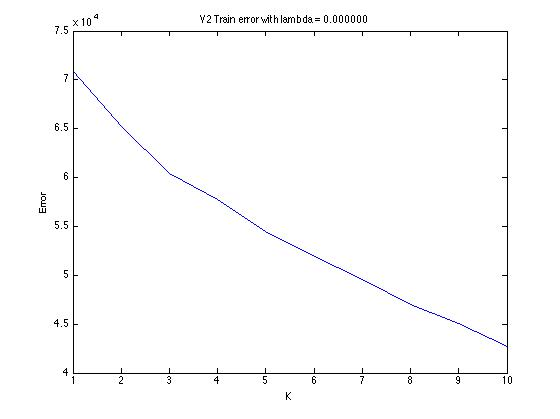
\includegraphics[scale=0.5]{TrainErrorLambda0-V2.jpg}
\caption{ $E_{tr}$ as of K with $\lambda=0.0$:}
\label{}
\end{figure}

\begin{figure}[H]
\centering
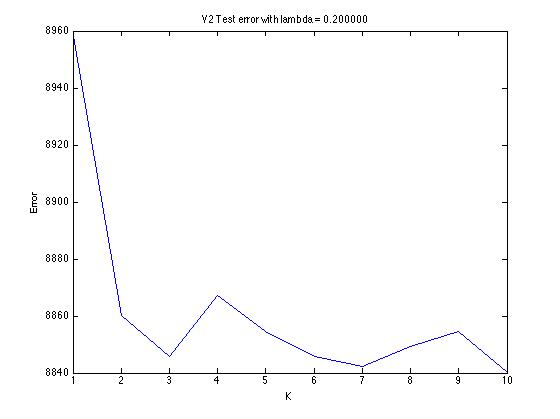
\includegraphics[scale=0.5]{TestErrorLambda02-V2.jpg}
\caption{ $E_{te}$ as of K with $\lambda=0.2$:}
\label{}
\end{figure}

\begin{figure}[H]
\centering
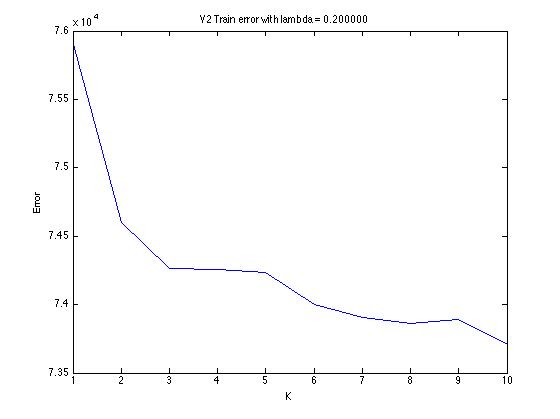
\includegraphics[scale=0.5]{TrainErrorLambda02-V2.jpg}
\caption{ $E_{tr}$ as of K with $\lambda=0.2$:}
\label{}
\end{figure}


\section{Question 2 -- PageRank Computation}
\subsection{(a)}
$r - r^{(k)} = \beta Mr - \beta Mr^{(k-1)} \\
=\beta M(r - r^{(k-1)}) \\
=\beta^2M^2(r - r^{(k-2)}) \\
=... \\
=\beta^kM^k(r - r^{(0)})$ \\
$M$ is stochastic, $\|M^kr\|_1 <= 1, \|M^kr^{(0)}\|_1 <= 1$ \\
So $\|r - r^{(k)}\|_1 <= \|\beta^k M^kr\|_1 + \|\beta^k M^kr^{(0)}\|_1 <= 2\beta^k$

\subsection{(b)}
Let $I$ be the number of iterations. \\
$\|r - r^{(I)}\|_1<= 2\beta^I <= \delta$\\
$I >= \log_\beta (\delta/2) = \frac{\log (2/\delta)}{\log (1/\beta)}$
We need iterate through every edge one time for each iteration. So total running time is: \\
$Im = m \frac{\log (2/\delta)}{\log (1/\beta)} = O({\frac{m}{\log (1/\beta)}})$



\subsection{(c)}
Let $c_j$ be the total number of visits at node j, Then $r_j = c_j\frac{1-\beta}{nR}$\\
Based on the algorithm, we have: $E[c_j] = \sum_{i->j} \beta \frac{E[c_i]}{deg(i)} + R$ \\
So, $E[\tilde{r_j}] = E[c_j]\frac{1-\beta}{nR} = \sum_{i->j} \beta \frac{E[c_i]\frac{1-\beta}{nR}}{deg(i)} + \frac{1-\beta}{n} \\
= \sum_{i->j} \beta \frac{E[c_i\frac{1-\beta}{nR}]}{deg(i)} + \frac{1-\beta}{n} \\
= \sum_{i->j} \beta \frac{E[\tilde{r_i}]}{deg(i)} + \frac{1-\beta}{n}$ \\
Which can be re-written as: $E[\tilde{r_j}] = \frac{1-\beta}{n}\textbf{1}^T + \beta ME[\tilde{r_j}]$ \\
We also have: $r_j = \frac{1-\beta}{n}\textbf{1}^T + \beta Mr_j$ \\
So $E[\tilde{r_j}] = r_j$


\subsection{(d)}
Expected run time of one random walker $E[w] = \sum_{i=1}^{\infty}i(1-\beta)\beta^{i-1}=\frac{1}{1-\beta}$\\
Expected running time of MC algorithm is: $E[w]\cdot nR = \frac{nR}{1-\beta}$

\subsection{(e)}
Power Iteration CPU time(40 Iterations): 13.341 ms\\
MC Algorithm with R=1, \\
\indent CPU time: 0.701 ms\\
\indent Average errors at Top 10, 30, 50, 100:\\
0.0028874375033 \\
0.00381215746702\\
0.00337883645241\\
0.00257711933559\\

\begin{figure}[H]
\centering
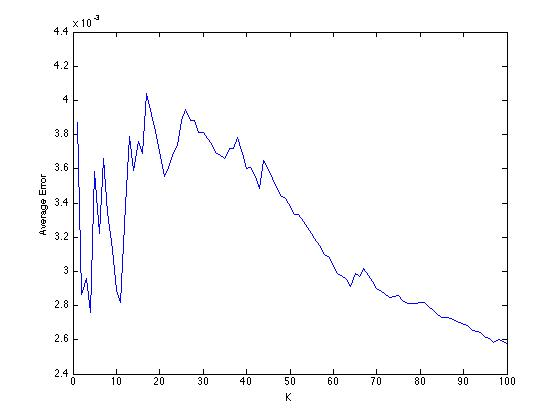
\includegraphics[scale=0.5]{q2-ErrorTopK-R1.jpg}
\caption{ Error at Top K, R = 1}
\label{}
\end{figure}

MC Algorithm with R=3, \\
\indent CPU time: 1.800 ms\\
\indent Average errors at Top 10, 30, 50, 100:\\
0.00258007835315 \\
0.00231232051217 \\
0.00199818494762 \\
0.00149559856577 \\

\begin{figure}[H]
\centering
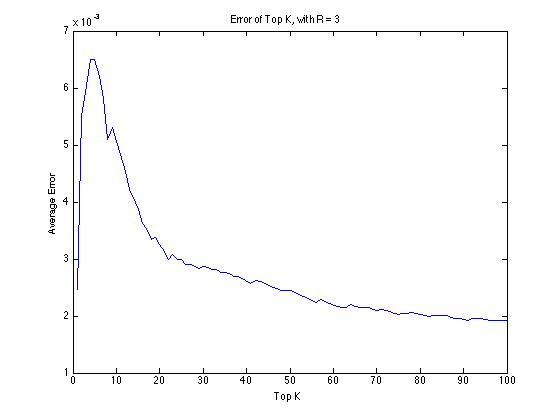
\includegraphics[scale=0.5]{q2-ErrorTopK-R3.jpg}
\caption{ Error at Top K, R = 3}
\label{}
\end{figure}

MC Algorithm with R=5, \\
\indent CPU time: 2.577 ms\\
\indent Average errors at Top 10, 30, 50, 100:\\
0.00299232555129 \\
0.00228341943338 \\
0.00180001027051 \\
0.00131482088127\\

\begin{figure}[H]
\centering
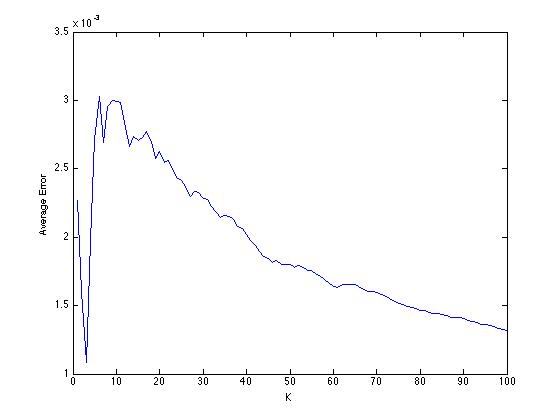
\includegraphics[scale=0.5]{q2-ErrorTopK-R5.jpg}
\caption{ Error at Top K, R = 5}
\label{}
\end{figure}

\section{Question 3 -- Similarity Ranking}
\subsection{(a)}
$s_A(camera, phone) = 0.343$\\
$s_A(camera, printer) = 0.0$\\

In first iteration, $s_A(camera, phone) = \\ C1\frac{s_B(nokia, nokia) +  s_B(nokia, apple) + s_B(kodak, nokia) + s_B(kodak, apple) + s_B(cannon, nokia) + s_B(cannon, apple)}{6} = \\ C1\frac{1 + 0 + 0 + 0 + 0 + 0}{6} = 0.133$ \\
Intermediate results (Nodes are indexed based on the order in graph, e.g. 'cameras' == 1, 'phones' == 2): \\
\begin{myenv}{0.8}
Round 1:\\ 
$s_A$:\\
(1, 2): 0.133333 \\
(1, 3): 0.000000 \\
(3, 3): 1.000000 \\
(2, 3): 0.000000 \\
(2, 2): 1.000000 \\
(1, 1): 1.000000 \\
$s_B$:\\
(1, 2): 0.000000 \\
(1, 3): 0.000000 \\
(3, 3): 1.000000 \\
(4, 5): 0.000000 \\
(4, 4): 1.000000 \\
(5, 5): 1.000000 \\
(1, 4): 0.000000 \\
(2, 4): 0.400000 \\
(1, 5): 0.000000 \\
(2, 3): 0.400000 \\
(2, 2): 1.000000 \\
(2, 5): 0.400000 \\
(3, 4): 0.000000 \\
(1, 1): 1.000000 \\
(3, 5): 0.800000 \\
Round 2:\\ 
$s_A$:\\
(1, 2): 0.293333 \\
(1, 3): 0.000000 \\
(3, 3): 1.000000 \\
(2, 3): 0.000000 \\
(2, 2): 1.000000 \\
(1, 1): 1.000000 \\
$s_B$:\\
(1, 2): 0.000000 \\
(1, 3): 0.000000 \\
(3, 3): 1.000000 \\
(4, 5): 0.106667 \\
(4, 4): 1.000000 \\
(5, 5): 1.000000 \\
(1, 4): 0.000000 \\
(2, 4): 0.453333 \\
(1, 5): 0.000000 \\
(2, 3): 0.453333 \\
(2, 2): 1.000000 \\
(2, 5): 0.453333 \\
(3, 4): 0.106667 \\
(1, 1): 1.000000 \\
(3, 5): 0.800000 \\
Round 3:\\ 
$s_A$:\\
(1, 2): 0.343111 \\
(1, 3): 0.000000 \\
(3, 3): 1.000000 \\
(2, 3): 0.000000 \\
(2, 2): 1.000000 \\
(1, 1): 1.000000 \\
$s_B$:\\
(1, 2): 0.000000 \\
(1, 3): 0.000000 \\
(3, 3): 1.000000 \\
(4, 5): 0.234667 \\
(4, 4): 1.000000 \\
(5, 5): 1.000000 \\
(1, 4): 0.000000 \\
(2, 4): 0.517333 \\
(1, 5): 0.000000 \\
(2, 3): 0.517333 \\
(2, 2): 1.000000 \\
(2, 5): 0.517333 \\
(3, 4): 0.234667 \\
(1, 1): 1.000000 \\
(3, 5): 0.800000 \\
\end{myenv}

\subsection{(b)}
Similarity equation incorporating link weights:\\
$s_A(X, Y) = C1\frac{ 
  \sum\limits_{i=1}^{|O(X)|} \sum\limits_{j=1}^{|O(Y)|} 
    s_B(O_i(X), O_j(Y))\cdot W_i(X)\cdot W_j(Y)
  }{
   \sum\limits_{i=1}^{|O(X)|} \sum\limits_{j=1}^{|O(Y)|}
    W_i(X)\cdot W_j(Y)
  } $ \\
Where $W_i(X)$ is the weight of the $i_{th}$ edge originating from $X$.
Similarly, we define $s_B$ as following: \\
$s_B(x, y) = C2\frac{ 
  \sum\limits_{i=1}^{|I(x)|} \sum\limits_{j=1}^{|I(y)|} 
    s_A(I_i(x), I_j(y))\cdot w_i(x)\cdot w_j(y)
  }{
    \sum\limits_{i=1}^{|I(x)|} \sum\limits_{j=1}^{|I(y)|} 
    w_i(x)\cdot w_j(y)
  } $ \\
Where $w_i(x)$ is the weight of the $i_{th}$ edge originating from $x$.

\subsection{(c)}
In $K_{2,1}$, $s_A(1, 2) = 0.800$ \\
In $K_{2,2}$, $s_A(1, 2) = 0.624$ \\

For $K_{2,1}$: \\

If first iteration, \\
$s_A(1, 2) =  \\ C1\frac{s_B(1, 1)}{1} =\\ C1\frac{1}{1} = 0.8$ \\
$s_A(1, 1) =  1$ \\
$s_A(2, 2) =  1$ \\
$s_B(1, 1) =  1$ \\


Intermediate results: \\

\begin{myenv}{0.8}
Round 1:\\ 
$s_A$:\\
(1, 2): 0.800000 \\
(1, 1): 1.000000 \\
(2, 2): 1.000000 \\
$s_B$:\\
(1, 1): 1.000000 \\
Round 2:\\ 
$s_A$:\\
(1, 2): 0.800000 \\
(1, 1): 1.000000 \\
(2, 2): 1.000000 \\
$s_B$:\\
(1, 1): 1.000000 \\
Round 3:\\ 
$s_A$:\\
(1, 2): 0.800000 \\
(1, 1): 1.000000 \\
(2, 2): 1.000000 \\
$s_B$:\\
(1, 1): 1.000000 \\
\end{myenv}

For $K_{2,2}$: \\

If first iteration, \\
$s_A(1, 2) =  \\ C1\frac{s_B(1, 1) + s_B(1, 2) + s_B(2, 1) + s_B(2, 2)}{4} =\\ C1\frac{1 + 0 + 0 + 1}{4} = 0.4$ \\
$s_A(1, 1) =  1$ \\
$s_A(2, 2) =  1$ \\
$s_A(2, 1) =  s_A(1, 2) = 0.4$ \\

$s_B(1, 2) =  \\ C2\frac{s_A(1, 1) + s_A(1, 2) + s_A(2, 1) + s_A(2, 2)}{4} =\\ C2\frac{1 + 0 + 0 + 1}{4} = 0.4$ \\
$s_B(1, 1) =  1$ \\
$s_B(2, 2) =  1$ \\
$s_B(2, 1) =  s_B(1, 2) = 0.4$ \\

Intermediate results: \\

\begin{myenv}{0.8}
Round 1:\\ 
$s_A$:\\
(1, 2): 0.400000 \\
(1, 1): 1.000000 \\
(2, 2): 1.000000 \\
$s_B$:\\
(1, 2): 0.400000 \\
(1, 1): 1.000000 \\
(2, 2): 1.000000 \\
Round 2:\\ 
$s_A$:\\
(1, 2): 0.560000 \\
(1, 1): 1.000000 \\
(2, 2): 1.000000 \\
$s_B$:\\
(1, 2): 0.560000 \\
(1, 1): 1.000000 \\
(2, 2): 1.000000 \\
Round 3:\\ 
$s_A$:\\
(1, 2): 0.624000 \\
(1, 1): 1.000000 \\
(2, 2): 1.000000 \\
$s_B$:\\
(1, 2): 0.624000 \\
(1, 1): 1.000000 \\
(2, 2): 1.000000 \\
\end{myenv}

\subsection{(d)}
Update the equations as:\\
$N_A(X, Y) = |O(X)| * |O(Y)|, \\
s_A(X, Y) = \frac{ (1-(1-C1)^{N_A(X, Y)})}
 {N_A(X, Y)} \sum\limits_{i=1}^{|O(X)|} \sum\limits_{j=1}^{|O(Y)|} 
    s_B(O_i(X), O_j(Y))$ \\

$N_B(x, y) = |I(x)| * |I(y)|, \\
s_B(x, y) = \frac{ (1-(1-C2)^{N_B(x, y)})}
 {N_B(X, Y)} \sum\limits_{i=1}^{|I(x)|} \sum\limits_{j=1}^{|I(y)|} 
    s_A(I_i(x), I_j(y))$ \\
    
The algorithm will converge. And final values are symmetric, and between [0, 1](Replaced C1/C2 with another const $(1-(1-C1)^{N_A(X, Y)})$ and $(1-(1-C1)^{N_A(X, Y)})$ that varies depending on the number of supporting evidences. More support, higher C1/C2) \\

Converged value of $s_A(1, 2)$ for $K_{2,1}$: \\
 0.49107427590144004 \\
and for $K_{2,2}$: \\
0.996805111821086 \\

The algorithm assigns higher score for $s_A(1, 2)$ in $K_{2,2}$ since there are more support.

\subsection{(e)}
Suppose we have two random walkers, one starting at $x \in A$, one starting at $y \in A$, in each iteration, if the walkers are in $A$, the process terminates with probability of (1 - C1), otherwise they walk to one of their neighbor nodes in $B$ with uniform probability respectively. If the walkers are in $B$,  the process terminates with probability of (1 - C2), otherwise  they walk to one of their neighbor nodes in $A$ with uniform probability respectively. Then $s_A(x, y)$ is the probability that the two random walkers from $x, y$ meet each other at some time, (at any round of the iteration).

\section{Question 4 -- Dense Communities in Networks}
\subsection{(a)}
\subsubsection{(i)}
Suppose $|A(S)| < \frac{\epsilon}{1+\epsilon}|S|$, \\
We denote $S\backslash A(S)$ as $B(S)$ \\
Then $|B(S)| = |\{i \in S | deg_s(i) > 2(1 + \epsilon)\rho(S)\}| > \frac{1}{1 + \epsilon}|S|$ \\
$|E[B(S)]| \ge |B(S)| \cdot 2(1 + \epsilon)\rho(S)/2 > \frac{1}{1 + \epsilon}|S| \cdot (1 + \epsilon)\frac{|E[S]|}{|S|} = |E[S]|$, which is impossible. \\
So $|A(S)| \ge \frac{\epsilon}{1+\epsilon}|S|$

\subsubsection{(ii)}
We denote $S$ in the $i_{th}$ iteration as $S_i$\\
Based on the proof in $\textbf{i}$, we have: $|S_{i+1}| < \frac{1}{1 + \epsilon}|S|$ \\
$|S_k| < \frac{1}{(1 + \epsilon)^k}|S| = \frac{1}{(1 + \epsilon)^k}n$ \\
 $S_k \ne  \emptyset$, So $|S_k| \ge 1$, $k < log_{1+\epsilon}(n)$
 
 \subsection{(b)}
 \subsubsection{(i)}
 If $\exists v \in S^* | deg_{S^*}(v) < \rho^*(G)$ \\
We can remove $v$ from $S^*$, let the resulting set be $S^\prime = S^*\backslash \{v\}$ \\
$\rho(S^\prime) = \frac{|E[S^\prime]|}{|S^\prime|} = \frac{|E[S^*]| - deg_{S^*}(v)}{|S^*| - 1}$ \\
Since $deg_{S^*}(v) < \rho^*(G) = \frac{|E[S^*]|}{|S^*|}$, \\
$\rho(S^\prime) = \frac{|E[S^*]| - deg_{S^*}(v)}{|S^*| - 1} > \frac{|E[S^*]|}{|S^*|} $ \\
$S^\prime$ is 'denser' than $S^*$. Which is contrary to the statement that $S^*$ is the densest subgrapgh of $G$. \\
So such $v$ doesn't exist.

 \subsubsection{(ii)}
In the first iteration of the while loop in which there exists a node $v \in S^* \cap A(S)$, Since $v \in S^*$, base on proof in $\textbf{i}$, we have $deg_{S^*}(v) \ge \rho^*(G)$ \\
Since $v \in A(S)$, we have $deg_{S}(v) \le 2(1+\epsilon)\rho(S)$ \\
$A(S) \in S$, So $S^* \cap A(S) \in S$, So $deg_{S^*}(v) \le deg_S(v)$ \\
$2(1+\epsilon)\rho(S) \ge deg_{S}(v) \ge deg_{S^*}(v) \ge \rho^*(G)$ \\
In conclusion, $2(1+\epsilon)\rho(S) \ge \rho^*(G)$

 \subsubsection{(iii)}
There should be at least 1 iteration (Assume in $j_{th}$ iteration) in which there exist node $v$ such that $v \in S^* \cap A(S)$. \\
Then $2(1+\epsilon)\rho(S_j) \ge \rho^*(G)$ \\
$\rho(\bar S) = \max\limits_{i=1}^{Num Iter}\{ \rho(S_i)\} \ge \rho(S_j) \ge \frac{1}{2(1+\epsilon)}\rho^*(G)$

 \subsection{(c)}
  \subsubsection{(i)}
 Number of iterations when $\epsilon = \{0.1, 0.5, 1, 2\}$ are: \\
  \{7, 5, 4, 3\}
 Corresponding theoretical bounds are: \\
 \{137, 32, 18, 11\}
 

   \begin{figure}[H]
\centering
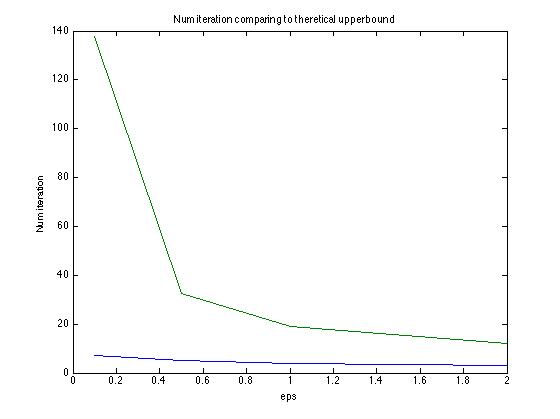
\includegraphics[scale=0.5]{q4-NumIterations.jpg}
\caption{ Num iterations and bounds }
\label{}
\end{figure}

\subsubsection{(ii)}


\begin{figure}[H]
\centering
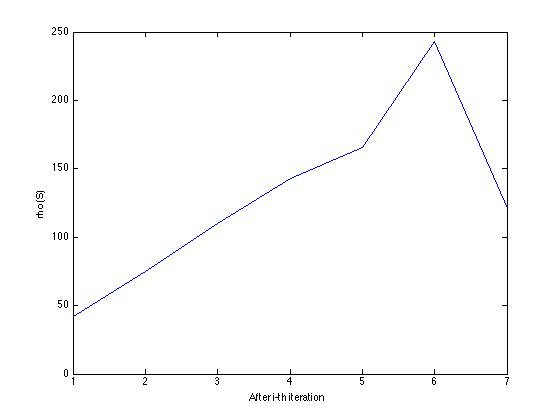
\includegraphics[scale=0.5]{q4-RhoSi.jpg}
\caption{ $\rho(S_i)$ as of $i$ }
\label{}
\end{figure}


\begin{figure}[H]
\centering
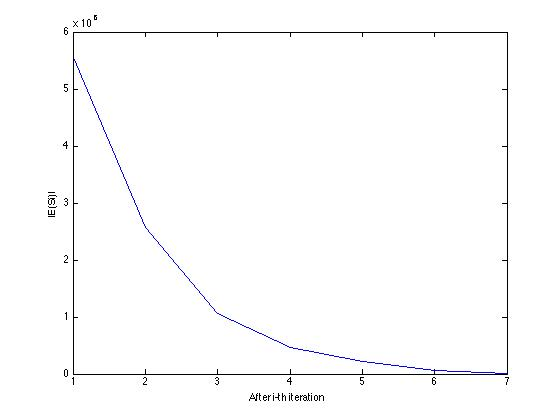
\includegraphics[scale=0.5]{q4-ESi.jpg}
\caption{ $|E(S_i)|$ as of $i$ }
\label{}
\end{figure}


\begin{figure}[H]
\centering
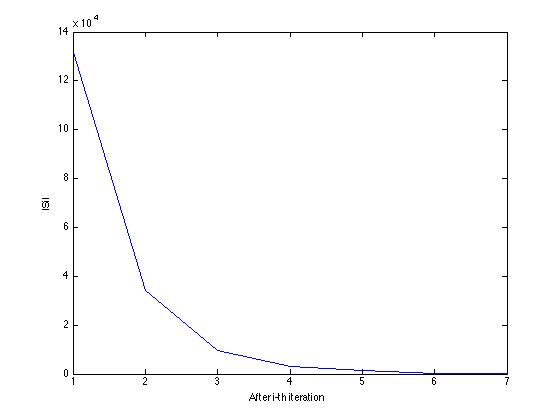
\includegraphics[scale=0.5]{q4-Si.jpg}
\caption{ $|S_i|$ as of $i$ }
\label{}
\end{figure}

\subsubsection{(iii)}

The plot of $\rho(\bar S_j), |E[\bar S_j]|$ and $|\bar S_j|$: \\

\begin{figure}[H]
\centering
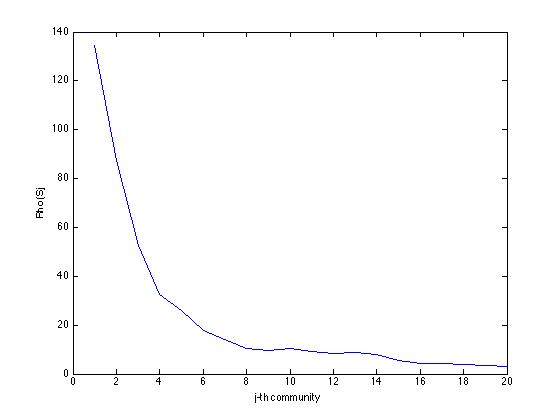
\includegraphics[scale=0.5]{q4c-rho.jpg}
\caption{ $\rho(\bar S_j)$ as of $j$}
\label{}
\end{figure}

\begin{figure}[H]
\centering
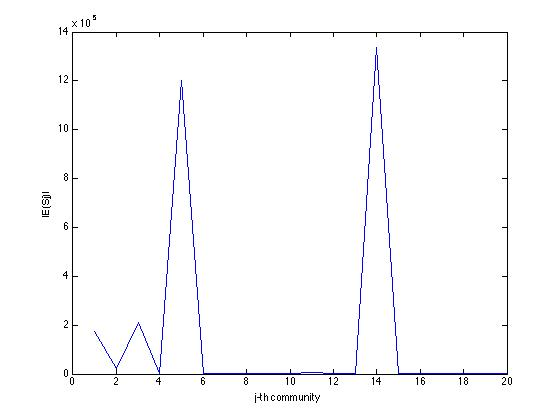
\includegraphics[scale=0.5]{q4c-esi.jpg}
\caption{ $|E[\bar S_j]|$ as of $j$}
\label{}
\end{figure}

\begin{figure}[H]
\centering
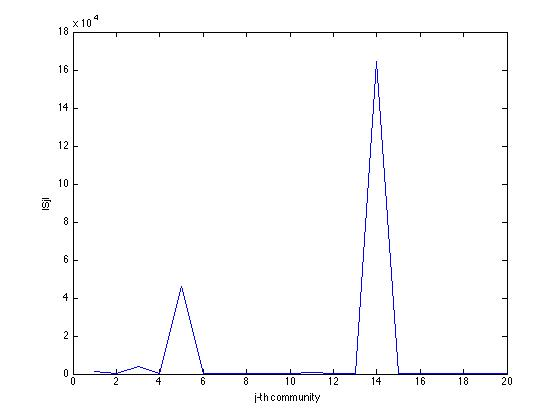
\includegraphics[scale=0.5]{q4c-si.jpg}
\caption{ $|\bar S_j|$ as of $j$}
\label{}
\end{figure}

The code:

\begin{myenv}{0.8}
\begin{verbatim}
from collections import defaultdict
import copy
import itertools
from optparse import OptionParser
import random
import sets
import sys
import time

def preprocess(graph_file, removed):
  f = open(graph_file)
  V = sets.Set()
  num_edge = 0
  for line in f:
    a, b = line.strip().split('\t')
    if removed and ((a in removed) or (b in removed)):
      continue
    if a not in V:
      V.add(a)
    if b not in V:
      V.add(b)
    num_edge += 1
  f.close()
  return V, num_edge

def count_edge(graph_file, S):
  f = open(graph_file)
  count = 0
  for line in f:
    a, b = line.strip().split('\t')
    if (a in S) and (b in S):
      count += 1
  f.close()
  return count

def find_dense(graph_file, eps, removed=None):
  V, e = preprocess(graph_file, removed)
  if len(V) == 0:
    return None, None, None, None, None
  S_bar = copy.copy(V)
  rho_S_bar = float(e) / len(V)
  S = copy.copy(V)
  num_iter = 0
  list_rho = []
  list_num_edge = []
  list_size_s = []
  while len(S) > 0:
    num_iter += 1
    deg = defaultdict(int)
    num_edge = 0
    f = open(graph_file)
    for line in f:
      a, b = line.strip().split('\t')
      if removed and ((a in removed) or (b in removed)):
        continue
      if (a not in S) or (b not in S):
        continue
      deg[a] += 1
      deg[b] += 1
      num_edge += 1
    f.close()
    rho_S = float(num_edge) / len(S)

    A = sets.Set()
    for v in S:
      if deg[v] <= 2 * (1 + eps) * rho_S:
        A.add(v)
    S.difference_update(A)
    num_edge = count_edge(graph_file, S)
    if len(S) == 0:
      break
    rho_S = float(num_edge) / len(S)
    if rho_S > rho_S_bar:
      rho_S_bar = rho_S
      S_bar = copy.copy(S)

    list_rho.append(rho_S)
    list_num_edge.append(num_edge)
    list_size_s.append(len(S))
  return S_bar, num_iter, list_rho, list_num_edge, list_size_s

def main():
  parser = OptionParser()
  parser.add_option("-f", "--file", dest="file", type="string",
                    help="File containing the graph.")
  (options, args) = parser.parse_args()

  for eps in [0.05, 0.1, 0.5, 1, 2]:
    S_bar, num_iter, list_rho, list_num_edge, list_size_s = find_dense(options.file, eps)
    print "Eps: %f, num iteration: %d" % (eps, num_iter)
    print list_rho
    print list_num_edge
    print list_size_s

  removed = sets.Set()
  eps = 0.05
  list_rho = []
  list_num_edge = []
  list_size_s = []
  for j in xrange(1, 21):
    print "%d-th iter" % j
    S_bar, t1, t2, t3, t4 = find_dense(options.file, eps, removed)
    if not S_bar:
      print "Remaining graph is empty"
      break
    num_edge = count_edge(options.file, S_bar)
    print "rho: %f" % (float(num_edge) / len(S_bar))
    list_rho.append(float(num_edge) / len(S_bar))
    print "num_edge: %d" % num_edge
    list_num_edge.append(num_edge)
    print "size_S_bar: %d" % len(S_bar)
    list_size_s.append(len(S_bar))
    removed = removed.union(S_bar)
    print S_bar
  print list_rho
  print list_num_edge
  print list_size_s

if __name__ == '__main__':
  main()
\end{verbatim}
\end{myenv}

\end{document}